% Options for packages loaded elsewhere
\PassOptionsToPackage{unicode}{hyperref}
\PassOptionsToPackage{hyphens}{url}
%
\documentclass[
]{article}
\usepackage{amsmath,amssymb}
\usepackage{iftex}
\ifPDFTeX
  \usepackage[T1]{fontenc}
  \usepackage[utf8]{inputenc}
  \usepackage{textcomp} % provide euro and other symbols
\else % if luatex or xetex
  \usepackage{unicode-math} % this also loads fontspec
  \defaultfontfeatures{Scale=MatchLowercase}
  \defaultfontfeatures[\rmfamily]{Ligatures=TeX,Scale=1}
\fi
\usepackage{lmodern}
\ifPDFTeX\else
  % xetex/luatex font selection
\fi
% Use upquote if available, for straight quotes in verbatim environments
\IfFileExists{upquote.sty}{\usepackage{upquote}}{}
\IfFileExists{microtype.sty}{% use microtype if available
  \usepackage[]{microtype}
  \UseMicrotypeSet[protrusion]{basicmath} % disable protrusion for tt fonts
}{}
\makeatletter
\@ifundefined{KOMAClassName}{% if non-KOMA class
  \IfFileExists{parskip.sty}{%
    \usepackage{parskip}
  }{% else
    \setlength{\parindent}{0pt}
    \setlength{\parskip}{6pt plus 2pt minus 1pt}}
}{% if KOMA class
  \KOMAoptions{parskip=half}}
\makeatother
\usepackage{xcolor}
\usepackage[margin=1in]{geometry}
\usepackage{color}
\usepackage{fancyvrb}
\newcommand{\VerbBar}{|}
\newcommand{\VERB}{\Verb[commandchars=\\\{\}]}
\DefineVerbatimEnvironment{Highlighting}{Verbatim}{commandchars=\\\{\}}
% Add ',fontsize=\small' for more characters per line
\usepackage{framed}
\definecolor{shadecolor}{RGB}{248,248,248}
\newenvironment{Shaded}{\begin{snugshade}}{\end{snugshade}}
\newcommand{\AlertTok}[1]{\textcolor[rgb]{0.94,0.16,0.16}{#1}}
\newcommand{\AnnotationTok}[1]{\textcolor[rgb]{0.56,0.35,0.01}{\textbf{\textit{#1}}}}
\newcommand{\AttributeTok}[1]{\textcolor[rgb]{0.13,0.29,0.53}{#1}}
\newcommand{\BaseNTok}[1]{\textcolor[rgb]{0.00,0.00,0.81}{#1}}
\newcommand{\BuiltInTok}[1]{#1}
\newcommand{\CharTok}[1]{\textcolor[rgb]{0.31,0.60,0.02}{#1}}
\newcommand{\CommentTok}[1]{\textcolor[rgb]{0.56,0.35,0.01}{\textit{#1}}}
\newcommand{\CommentVarTok}[1]{\textcolor[rgb]{0.56,0.35,0.01}{\textbf{\textit{#1}}}}
\newcommand{\ConstantTok}[1]{\textcolor[rgb]{0.56,0.35,0.01}{#1}}
\newcommand{\ControlFlowTok}[1]{\textcolor[rgb]{0.13,0.29,0.53}{\textbf{#1}}}
\newcommand{\DataTypeTok}[1]{\textcolor[rgb]{0.13,0.29,0.53}{#1}}
\newcommand{\DecValTok}[1]{\textcolor[rgb]{0.00,0.00,0.81}{#1}}
\newcommand{\DocumentationTok}[1]{\textcolor[rgb]{0.56,0.35,0.01}{\textbf{\textit{#1}}}}
\newcommand{\ErrorTok}[1]{\textcolor[rgb]{0.64,0.00,0.00}{\textbf{#1}}}
\newcommand{\ExtensionTok}[1]{#1}
\newcommand{\FloatTok}[1]{\textcolor[rgb]{0.00,0.00,0.81}{#1}}
\newcommand{\FunctionTok}[1]{\textcolor[rgb]{0.13,0.29,0.53}{\textbf{#1}}}
\newcommand{\ImportTok}[1]{#1}
\newcommand{\InformationTok}[1]{\textcolor[rgb]{0.56,0.35,0.01}{\textbf{\textit{#1}}}}
\newcommand{\KeywordTok}[1]{\textcolor[rgb]{0.13,0.29,0.53}{\textbf{#1}}}
\newcommand{\NormalTok}[1]{#1}
\newcommand{\OperatorTok}[1]{\textcolor[rgb]{0.81,0.36,0.00}{\textbf{#1}}}
\newcommand{\OtherTok}[1]{\textcolor[rgb]{0.56,0.35,0.01}{#1}}
\newcommand{\PreprocessorTok}[1]{\textcolor[rgb]{0.56,0.35,0.01}{\textit{#1}}}
\newcommand{\RegionMarkerTok}[1]{#1}
\newcommand{\SpecialCharTok}[1]{\textcolor[rgb]{0.81,0.36,0.00}{\textbf{#1}}}
\newcommand{\SpecialStringTok}[1]{\textcolor[rgb]{0.31,0.60,0.02}{#1}}
\newcommand{\StringTok}[1]{\textcolor[rgb]{0.31,0.60,0.02}{#1}}
\newcommand{\VariableTok}[1]{\textcolor[rgb]{0.00,0.00,0.00}{#1}}
\newcommand{\VerbatimStringTok}[1]{\textcolor[rgb]{0.31,0.60,0.02}{#1}}
\newcommand{\WarningTok}[1]{\textcolor[rgb]{0.56,0.35,0.01}{\textbf{\textit{#1}}}}
\usepackage{graphicx}
\makeatletter
\def\maxwidth{\ifdim\Gin@nat@width>\linewidth\linewidth\else\Gin@nat@width\fi}
\def\maxheight{\ifdim\Gin@nat@height>\textheight\textheight\else\Gin@nat@height\fi}
\makeatother
% Scale images if necessary, so that they will not overflow the page
% margins by default, and it is still possible to overwrite the defaults
% using explicit options in \includegraphics[width, height, ...]{}
\setkeys{Gin}{width=\maxwidth,height=\maxheight,keepaspectratio}
% Set default figure placement to htbp
\makeatletter
\def\fps@figure{htbp}
\makeatother
\setlength{\emergencystretch}{3em} % prevent overfull lines
\providecommand{\tightlist}{%
  \setlength{\itemsep}{0pt}\setlength{\parskip}{0pt}}
\setcounter{secnumdepth}{-\maxdimen} % remove section numbering
\ifLuaTeX
  \usepackage{selnolig}  % disable illegal ligatures
\fi
\usepackage{bookmark}
\IfFileExists{xurl.sty}{\usepackage{xurl}}{} % add URL line breaks if available
\urlstyle{same}
\hypersetup{
  pdftitle={Case Solution 1 Group 5},
  pdfauthor={Balint Keller},
  hidelinks,
  pdfcreator={LaTeX via pandoc}}

\title{Case Solution 1 Group 5}
\author{Balint Keller}
\date{2025-03-28}

\begin{document}
\maketitle

\subsubsection{Hypothesis Testing}\label{hypothesis-testing}

\textbf{H0:} B2 = 0 → Education has no effect on wages.

\textbf{H1:} B2 \textgreater{} 0 → Education has a positive effect on
wages.

One-sided hypotheses are appropriate in this case because education is
expected to increase earnings (according to economic theories).\\
In addition, there's often little reason to test whether more education
reduces wages because that result is counterintuitive.

\begin{Shaded}
\begin{Highlighting}[]
\FunctionTok{head}\NormalTok{(df)}
\end{Highlighting}
\end{Shaded}

\begin{verbatim}
##       WAGE EDUC AGE RACE SMSA MARRIED REGION QOB
## 1 580.1000    9  45    0    0       1      9   3
## 2 642.2115   17  47    0    0       1      3   4
## 3 577.0192   12  42    0    0       1      7   2
## 4 999.1346   10  43    0    0       1      3   2
## 5 307.7885   12  41    0    0       1      6   3
## 6 280.1000   12  40    1    0       1      5   2
\end{verbatim}

\begin{Shaded}
\begin{Highlighting}[]
\CommentTok{\#Creation of dummy vars for the regions and QOBs}
\NormalTok{df }\OtherTok{\textless{}{-}}\NormalTok{ df }\SpecialCharTok{\%\textgreater{}\%}
  \FunctionTok{mutate}\NormalTok{(}
    \AttributeTok{REGION1 =} \FunctionTok{as.integer}\NormalTok{(REGION }\SpecialCharTok{==} \DecValTok{1}\NormalTok{),}
    \AttributeTok{REGION2 =} \FunctionTok{as.integer}\NormalTok{(REGION }\SpecialCharTok{==} \DecValTok{2}\NormalTok{),}
    \AttributeTok{REGION3 =} \FunctionTok{as.integer}\NormalTok{(REGION }\SpecialCharTok{==} \DecValTok{3}\NormalTok{),}
    \AttributeTok{REGION4 =} \FunctionTok{as.integer}\NormalTok{(REGION }\SpecialCharTok{==} \DecValTok{4}\NormalTok{),}
    \AttributeTok{REGION5 =} \FunctionTok{as.integer}\NormalTok{(REGION }\SpecialCharTok{==} \DecValTok{5}\NormalTok{),}
    \AttributeTok{REGION6 =} \FunctionTok{as.integer}\NormalTok{(REGION }\SpecialCharTok{==} \DecValTok{6}\NormalTok{),}
    \AttributeTok{REGION7 =} \FunctionTok{as.integer}\NormalTok{(REGION }\SpecialCharTok{==} \DecValTok{7}\NormalTok{),}
    \AttributeTok{REGION8 =} \FunctionTok{as.integer}\NormalTok{(REGION }\SpecialCharTok{==} \DecValTok{8}\NormalTok{),}
    \AttributeTok{REGION9 =} \FunctionTok{as.integer}\NormalTok{(REGION }\SpecialCharTok{==} \DecValTok{9}\NormalTok{),}

    \AttributeTok{QOB1 =} \FunctionTok{as.integer}\NormalTok{(QOB }\SpecialCharTok{==} \DecValTok{1}\NormalTok{),}
    \AttributeTok{QOB2 =} \FunctionTok{as.integer}\NormalTok{(QOB }\SpecialCharTok{==} \DecValTok{2}\NormalTok{),}
    \AttributeTok{QOB3 =} \FunctionTok{as.integer}\NormalTok{(QOB }\SpecialCharTok{==} \DecValTok{3}\NormalTok{),}
    \AttributeTok{QOB4 =} \FunctionTok{as.integer}\NormalTok{(QOB }\SpecialCharTok{==} \DecValTok{4}\NormalTok{)}
\NormalTok{  )}
\end{Highlighting}
\end{Shaded}

\begin{Shaded}
\begin{Highlighting}[]
\FunctionTok{summary}\NormalTok{(df)}
\end{Highlighting}
\end{Shaded}

\begin{verbatim}
##       WAGE                EDUC            AGE             RACE       
##  Min.   :    0.096   Min.   : 0.00   Min.   :40.00   Min.   :0.0000  
##  1st Qu.:  278.558   1st Qu.:12.00   1st Qu.:42.00   1st Qu.:0.0000  
##  Median :  384.712   Median :12.00   Median :45.00   Median :0.0000  
##  Mean   :  436.524   Mean   :12.71   Mean   :44.68   Mean   :0.0832  
##  3rd Qu.:  520.100   3rd Qu.:15.00   3rd Qu.:47.00   3rd Qu.:0.0000  
##  Max.   :10167.500   Max.   :20.00   Max.   :50.00   Max.   :1.0000  
##       SMSA           MARRIED           REGION           QOB       
##  Min.   :0.0000   Min.   :0.0000   Min.   :1.000   Min.   :1.000  
##  1st Qu.:0.0000   1st Qu.:1.0000   1st Qu.:3.000   1st Qu.:1.000  
##  Median :0.0000   Median :1.0000   Median :5.000   Median :3.000  
##  Mean   :0.1813   Mean   :0.8609   Mean   :4.767   Mean   :2.502  
##  3rd Qu.:0.0000   3rd Qu.:1.0000   3rd Qu.:7.000   3rd Qu.:3.000  
##  Max.   :1.0000   Max.   :1.0000   Max.   :9.000   Max.   :4.000  
##     REGION1          REGION2          REGION3          REGION4      
##  Min.   :0.0000   Min.   :0.0000   Min.   :0.0000   Min.   :0.0000  
##  1st Qu.:0.0000   1st Qu.:0.0000   1st Qu.:0.0000   1st Qu.:0.0000  
##  Median :0.0000   Median :0.0000   Median :0.0000   Median :0.0000  
##  Mean   :0.0549   Mean   :0.1584   Mean   :0.1949   Mean   :0.0732  
##  3rd Qu.:0.0000   3rd Qu.:0.0000   3rd Qu.:0.0000   3rd Qu.:0.0000  
##  Max.   :1.0000   Max.   :1.0000   Max.   :1.0000   Max.   :1.0000  
##     REGION5          REGION6         REGION7          REGION8      
##  Min.   :0.0000   Min.   :0.000   Min.   :0.0000   Min.   :0.0000  
##  1st Qu.:0.0000   1st Qu.:0.000   1st Qu.:0.0000   1st Qu.:0.0000  
##  Median :0.0000   Median :0.000   Median :0.0000   Median :0.0000  
##  Mean   :0.1773   Mean   :0.064   Mean   :0.0995   Mean   :0.0494  
##  3rd Qu.:0.0000   3rd Qu.:0.000   3rd Qu.:0.0000   3rd Qu.:0.0000  
##  Max.   :1.0000   Max.   :1.000   Max.   :1.0000   Max.   :1.0000  
##     REGION9            QOB1             QOB2             QOB3       
##  Min.   :0.0000   Min.   :0.0000   Min.   :0.0000   Min.   :0.0000  
##  1st Qu.:0.0000   1st Qu.:0.0000   1st Qu.:0.0000   1st Qu.:0.0000  
##  Median :0.0000   Median :0.0000   Median :0.0000   Median :0.0000  
##  Mean   :0.1284   Mean   :0.2533   Mean   :0.2354   Mean   :0.2674  
##  3rd Qu.:0.0000   3rd Qu.:1.0000   3rd Qu.:0.0000   3rd Qu.:1.0000  
##  Max.   :1.0000   Max.   :1.0000   Max.   :1.0000   Max.   :1.0000  
##       QOB4       
##  Min.   :0.0000  
##  1st Qu.:0.0000  
##  Median :0.0000  
##  Mean   :0.2439  
##  3rd Qu.:0.0000  
##  Max.   :1.0000
\end{verbatim}

\begin{Shaded}
\begin{Highlighting}[]
\FunctionTok{describe}\NormalTok{(df)}
\end{Highlighting}
\end{Shaded}

\begin{verbatim}
##         vars     n   mean     sd median trimmed    mad  min     max   range
## WAGE       1 10000 436.52 295.37 384.71  401.88 173.27  0.1 10167.5 10167.4
## EDUC       2 10000  12.71   3.28  12.00   12.72   2.97  0.0    20.0    20.0
## AGE        3 10000  44.68   2.93  45.00   44.67   4.45 40.0    50.0    10.0
## RACE       4 10000   0.08   0.28   0.00    0.00   0.00  0.0     1.0     1.0
## SMSA       5 10000   0.18   0.39   0.00    0.10   0.00  0.0     1.0     1.0
## MARRIED    6 10000   0.86   0.35   1.00    0.95   0.00  0.0     1.0     1.0
## REGION     7 10000   4.77   2.46   5.00    4.65   2.97  1.0     9.0     8.0
## QOB        8 10000   2.50   1.12   3.00    2.50   1.48  1.0     4.0     3.0
## REGION1    9 10000   0.05   0.23   0.00    0.00   0.00  0.0     1.0     1.0
## REGION2   10 10000   0.16   0.37   0.00    0.07   0.00  0.0     1.0     1.0
## REGION3   11 10000   0.19   0.40   0.00    0.12   0.00  0.0     1.0     1.0
## REGION4   12 10000   0.07   0.26   0.00    0.00   0.00  0.0     1.0     1.0
## REGION5   13 10000   0.18   0.38   0.00    0.10   0.00  0.0     1.0     1.0
## REGION6   14 10000   0.06   0.24   0.00    0.00   0.00  0.0     1.0     1.0
## REGION7   15 10000   0.10   0.30   0.00    0.00   0.00  0.0     1.0     1.0
## REGION8   16 10000   0.05   0.22   0.00    0.00   0.00  0.0     1.0     1.0
## REGION9   17 10000   0.13   0.33   0.00    0.04   0.00  0.0     1.0     1.0
## QOB1      18 10000   0.25   0.43   0.00    0.19   0.00  0.0     1.0     1.0
## QOB2      19 10000   0.24   0.42   0.00    0.17   0.00  0.0     1.0     1.0
## QOB3      20 10000   0.27   0.44   0.00    0.21   0.00  0.0     1.0     1.0
## QOB4      21 10000   0.24   0.43   0.00    0.18   0.00  0.0     1.0     1.0
##          skew kurtosis   se
## WAGE     7.39   170.46 2.95
## EDUC    -0.07     0.55 0.03
## AGE      0.05    -1.18 0.03
## RACE     3.02     7.11 0.00
## SMSA     1.65     0.74 0.00
## MARRIED -2.09     2.35 0.00
## REGION   0.35    -1.06 0.02
## QOB     -0.03    -1.35 0.01
## REGION1  3.91    13.27 0.00
## REGION2  1.87     1.50 0.00
## REGION3  1.54     0.37 0.00
## REGION4  3.28     8.74 0.00
## REGION5  1.69     0.85 0.00
## REGION6  3.56    10.69 0.00
## REGION7  2.68     5.16 0.00
## REGION8  4.16    15.29 0.00
## REGION9  2.22     2.93 0.00
## QOB1     1.13    -0.71 0.00
## QOB2     1.25    -0.44 0.00
## QOB3     1.05    -0.90 0.00
## QOB4     1.19    -0.58 0.00
\end{verbatim}

\begin{Shaded}
\begin{Highlighting}[]
\FunctionTok{cov}\NormalTok{(df)}
\end{Highlighting}
\end{Shaded}

\begin{verbatim}
##                  WAGE          EDUC          AGE          RACE          SMSA
## WAGE    87241.0836001  3.157684e+02  5.256929832 -1.049000e+01 -1.485766e+01
## EDUC      315.7684062  1.074171e+01 -0.667730053 -1.375518e-01 -1.882395e-01
## AGE         5.2569298 -6.677301e-01  8.591725483 -4.168257e-03 -2.355067e-02
## RACE      -10.4899998 -1.375518e-01 -0.004168257  7.628539e-02 -3.784538e-03
## SMSA      -14.8576552 -1.882395e-01 -0.023550665 -3.784538e-03  1.484452e-01
## MARRIED    10.1783750  2.177522e-02  0.021109281 -1.082796e-02  5.419372e-03
## REGION      8.8550412  2.740826e-01 -0.125475448  1.185719e-03  3.264616e-02
## QOB         2.3974020  1.174544e-01 -0.386878218 -3.758456e-03 -4.794949e-03
## REGION1    -0.8536330  1.648109e-02  0.016140984 -2.867967e-03 -1.753545e-03
## REGION2     3.8199259  4.274331e-02  0.009094829  1.421262e-03 -1.461938e-02
## REGION3     3.3789188 -4.004056e-02  0.006221992 -2.615942e-03 -3.735744e-03
## REGION4    -1.1378266 -4.941294e-04 -0.011381978 -3.590599e-03  1.183002e-02
## REGION5    -6.8153854 -5.376850e-02 -0.013634873  9.649605e-03  2.855796e-03
## REGION6    -3.9603260 -6.772837e-02  0.005963796  2.675468e-03  1.069787e-02
## REGION7    -1.9950947 -3.218602e-02  0.002769627  7.216722e-04 -1.239474e-03
## REGION8    -0.2171291  2.021066e-02 -0.016629443 -2.610341e-03  5.944374e-03
## REGION9     7.7805501  1.147825e-01  0.001455066 -2.783158e-03 -9.979918e-03
## QOB1       -0.8194058 -4.086161e-02  0.193104600 -1.745775e-04  2.876998e-03
## QOB2       -0.4775954  1.293153e-02 -0.063772357  2.514971e-03 -8.781078e-04
## QOB3        1.0160062 -2.073263e-02 -0.064890869 -7.477548e-04 -2.079828e-03
## QOB4        0.2809950  4.866271e-02 -0.064441374 -1.592639e-03  8.093809e-05
##               MARRIED       REGION           QOB       REGION1       REGION2
## WAGE    10.1783750456  8.855041195  2.3974019986 -0.8536330190  3.8199258573
## EDUC     0.0217752175  0.274082608  0.1174543854  0.0164810881  0.0427433143
## AGE      0.0211092809 -0.125475448 -0.3868782178  0.0161409841  0.0090948295
## RACE    -0.0108279628  0.001185719 -0.0037584558 -0.0028679668  0.0014212621
## SMSA     0.0054193719  0.032646165 -0.0047949495 -0.0017535454 -0.0146193819
## MARRIED  0.1197631663 -0.022112511 -0.0027859886 -0.0006634763 -0.0004666067
## REGION  -0.0221125113  6.064117412 -0.0024575458 -0.2068289829 -0.4383366337
## QOB     -0.0027859886 -0.002457546  1.2445208421  0.0009457846  0.0047995200
## REGION1 -0.0006634763 -0.206828983  0.0009457846  0.0518911791 -0.0086970297
## REGION2 -0.0004666067 -0.438336634  0.0047995200 -0.0086970297  0.1333227723
## REGION3  0.0019107811 -0.344422742 -0.0027205821 -0.0107010801 -0.0308752475
## REGION4  0.0018823082 -0.056150015 -0.0064397240 -0.0040190819 -0.0115960396
## REGION5  0.0005624862  0.041315032  0.0024133713 -0.0097347435 -0.0280871287
## REGION6  0.0015025503  0.078919892 -0.0026218622 -0.0035139514 -0.0101386139
## REGION7  0.0007405241  0.222205721  0.0044613961 -0.0054630963 -0.0157623762
## REGION8  0.0015716972  0.159726173 -0.0008939494 -0.0027123312 -0.0078257426
## REGION9 -0.0070402640  0.543571557  0.0000560456 -0.0070498650 -0.0203405941
## QOB1    -0.0005660266  0.004519352 -0.3804693169 -0.0009062606 -0.0028230023
## QOB2     0.0015442944 -0.013753175 -0.1181590759  0.0009766377  0.0022128613
## QOB3     0.0013954795  0.016405841  0.1332052605 -0.0001802780 -0.0007562356
## QOB4    -0.0023737474 -0.007172017  0.3654231323  0.0001099010  0.0013663766
##               REGION3       REGION4       REGION5       REGION6       REGION7
## WAGE     3.3789187829 -1.1378265754 -6.8153853707 -3.9603259637 -1.9950946778
## EDUC    -0.0400405641 -0.0004941294 -0.0537684968 -0.0677283728 -0.0321860186
## AGE      0.0062219922 -0.0113819782 -0.0136348735  0.0059637964  0.0027696270
## RACE    -0.0026159416 -0.0035905991  0.0096496050  0.0026754675  0.0007216722
## SMSA    -0.0037357436  0.0118300230  0.0028557956  0.0106978698 -0.0012394739
## MARRIED  0.0019107811  0.0018823082  0.0005624862  0.0015025503  0.0007405241
## REGION  -0.3444227423 -0.0561500150  0.0413150315  0.0789198920  0.2222057206
## QOB     -0.0027205821 -0.0064397240  0.0024133713 -0.0026218622  0.0044613961
## REGION1 -0.0107010801 -0.0040190819 -0.0097347435 -0.0035139514 -0.0054630963
## REGION2 -0.0308752475 -0.0115960396 -0.0280871287 -0.0101386139 -0.0157623762
## REGION3  0.1569296830 -0.0142681068 -0.0345592259 -0.0124748475 -0.0193944894
## REGION4 -0.0142681068  0.0678485449 -0.0129796580 -0.0046852685 -0.0072841284
## REGION5 -0.0345592259 -0.0129796580  0.1458792979 -0.0113483348 -0.0176431143
## REGION6 -0.0124748475 -0.0046852685 -0.0113483348  0.0599099910 -0.0063686369
## REGION7 -0.0193944894 -0.0072841284 -0.0176431143 -0.0063686369  0.0896087109
## REGION8 -0.0096290229 -0.0036164416 -0.0087594959 -0.0031619162 -0.0049157916
## REGION9 -0.0250276628 -0.0093998200 -0.0227675968 -0.0082184218 -0.0127770777
## QOB1     0.0014319732  0.0015585959  0.0007899890  0.0012889289 -0.0008034303
## QOB2     0.0003205721  0.0007687969 -0.0020366237 -0.0003656366 -0.0030226023
## QOB3    -0.0022164816  0.0002263426 -0.0007100910 -0.0005136514  0.0039940994
## QOB4     0.0004639364 -0.0025537354  0.0019567257 -0.0004096410 -0.0001680668
##               REGION8       REGION9          QOB1          QOB2          QOB3
## WAGE    -2.171291e-01  7.7805501010 -0.8194057861 -4.775954e-01  1.0160061545
## EDUC     2.021066e-02  0.1147825183 -0.0408616062  1.293153e-02 -0.0207326333
## AGE     -1.662944e-02  0.0014550655  0.1931046005 -6.377236e-02 -0.0648908691
## RACE    -2.610341e-03 -0.0027831583 -0.0001745775  2.514971e-03 -0.0007477548
## SMSA     5.944374e-03 -0.0099799180  0.0028769977 -8.781078e-04 -0.0020798280
## MARRIED  1.571697e-03 -0.0070402640 -0.0005660266  1.544294e-03  0.0013954795
## REGION   1.597262e-01  0.5435715572  0.0045193519 -1.375318e-02  0.0164058406
## QOB     -8.939494e-04  0.0000560456 -0.3804693169 -1.181591e-01  0.1332052605
## REGION1 -2.712331e-03 -0.0070498650 -0.0009062606  9.766377e-04 -0.0001802780
## REGION2 -7.825743e-03 -0.0203405941 -0.0028230023  2.212861e-03 -0.0007562356
## REGION3 -9.629023e-03 -0.0250276628  0.0014319732  3.205721e-04 -0.0022164816
## REGION4 -3.616442e-03 -0.0093998200  0.0015585959  7.687969e-04  0.0002263426
## REGION5 -8.759496e-03 -0.0227675968  0.0007899890 -2.036624e-03 -0.0007100910
## REGION6 -3.161916e-03 -0.0082184218  0.0012889289 -3.656366e-04 -0.0005136514
## REGION7 -4.915792e-03 -0.0127770777 -0.0008034303 -3.022602e-03  0.0039940994
## REGION8  4.696434e-02 -0.0063435944  0.0006870487 -2.876288e-05 -0.0011096710
## REGION9 -6.343594e-03  0.1119246325 -0.0012238424  1.174757e-03  0.0012659666
## QOB1     6.870487e-04 -0.0012238424  0.1891580258 -5.963278e-02 -0.0677391939
## QOB2    -2.876288e-05  0.0011747575 -0.0596327833  1.800048e-01 -0.0629522552
## QOB3    -1.109671e-03  0.0012659666 -0.0677391939 -6.295226e-02  0.1959168317
## QOB4     4.513851e-04 -0.0012168817 -0.0617860486 -5.741980e-02 -0.0652253825
##                  QOB4
## WAGE     2.809950e-01
## EDUC     4.866271e-02
## AGE     -6.444137e-02
## RACE    -1.592639e-03
## SMSA     8.093809e-05
## MARRIED -2.373747e-03
## REGION  -7.172017e-03
## QOB      3.654231e-01
## REGION1  1.099010e-04
## REGION2  1.366377e-03
## REGION3  4.639364e-04
## REGION4 -2.553735e-03
## REGION5  1.956726e-03
## REGION6 -4.096410e-04
## REGION7 -1.680668e-04
## REGION8  4.513851e-04
## REGION9 -1.216882e-03
## QOB1    -6.178605e-02
## QOB2    -5.741980e-02
## QOB3    -6.522538e-02
## QOB4     1.844312e-01
\end{verbatim}

\begin{Shaded}
\begin{Highlighting}[]
\FunctionTok{cor}\NormalTok{(df)}
\end{Highlighting}
\end{Shaded}

\begin{verbatim}
##                 WAGE         EDUC          AGE         RACE         SMSA
## WAGE     1.000000000  0.326190646  0.006071996 -0.128586174 -0.130558976
## EDUC     0.326190646  1.000000000 -0.069506286 -0.151952924 -0.149070326
## AGE      0.006071996 -0.069506286  1.000000000 -0.005148653 -0.020853549
## RACE    -0.128586174 -0.151952924 -0.005148653  1.000000000 -0.035563888
## SMSA    -0.130558976 -0.149070326 -0.020853549 -0.035563888  1.000000000
## MARRIED  0.099576370  0.019198364  0.020809977 -0.113282921  0.040644736
## REGION   0.012174363  0.033959480 -0.017383401  0.001743320  0.034408469
## QOB      0.007275775  0.032124139 -0.118313144 -0.012197973 -0.011155780
## REGION1 -0.012687145  0.022075089  0.024173695 -0.045583395 -0.019979620
## REGION2  0.035419485  0.035717362  0.008497716  0.014092931 -0.103918730
## REGION3  0.028877838 -0.030839760  0.005358420 -0.023908637 -0.024476059
## REGION4 -0.014789220 -0.000578807 -0.014907585 -0.049908666  0.117877877
## REGION5 -0.060413370 -0.042953090 -0.012179069  0.091472810  0.019406502
## REGION6 -0.054779843 -0.084427585  0.008312525  0.039575771  0.113439595
## REGION7 -0.022564612 -0.032806167  0.003156501  0.008728591 -0.010746803
## REGION8 -0.003392138  0.028455078 -0.026179022 -0.043610641  0.071193288
## REGION9  0.078738464  0.104683025  0.001483814 -0.030119960 -0.077424983
## QOB1    -0.006378611 -0.028665954  0.151474678 -0.001453299  0.017168965
## QOB2    -0.003811163  0.009299750 -0.051280256  0.021462005 -0.005371836
## QOB3     0.007771412 -0.014291636 -0.050015835 -0.006116495 -0.012195750
## QOB4     0.002215240  0.034573423 -0.051192621 -0.013427016  0.000489162
##              MARRIED        REGION           QOB      REGION1      REGION2
## WAGE     0.099576370  0.0121743634  0.0072757748 -0.012687145  0.035419485
## EDUC     0.019198364  0.0339594799  0.0321241395  0.022075089  0.035717362
## AGE      0.020809977 -0.0173834013 -0.1183131440  0.024173695  0.008497716
## RACE    -0.113282921  0.0017433201 -0.0121979735 -0.045583395  0.014092931
## SMSA     0.040644736  0.0344084693 -0.0111557799 -0.019979620 -0.103918730
## MARRIED  1.000000000 -0.0259473274 -0.0072163338 -0.008416219 -0.003692641
## REGION  -0.025947327  1.0000000000 -0.0008945749 -0.368706527 -0.487496834
## QOB     -0.007216334 -0.0008945749  1.0000000000  0.003721726  0.011782693
## REGION1 -0.008416219 -0.3687065272  0.0037217258  1.000000000 -0.104561551
## REGION2 -0.003692641 -0.4874968339  0.0117826926 -0.104561551  1.000000000
## REGION3  0.013937881 -0.3530656533 -0.0061561358 -0.118584601 -0.213454705
## REGION4  0.020881363 -0.0875378361 -0.0221613339 -0.067734483 -0.121923453
## REGION5  0.004255528  0.0439265864  0.0056640389 -0.111887330 -0.201399480
## REGION6  0.017738535  0.1309341865 -0.0096019435 -0.063023041 -0.113442761
## REGION7  0.007148294  0.3014368342  0.0133596348 -0.080115578 -0.144209678
## REGION8  0.020956712  0.2993010147 -0.0036976666 -0.054942936 -0.098898407
## REGION9 -0.060808526  0.6597966173  0.0001501681 -0.092506275 -0.166513184
## QOB1    -0.003760649  0.0042196844 -0.7841626724 -0.009147322 -0.017776517
## QOB2     0.010517836 -0.0131636730 -0.2496455947  0.010105193  0.014284332
## QOB3     0.009110159  0.0150514664  0.2697642622 -0.001787970 -0.004679173
## QOB4    -0.015971865 -0.0067817267  0.7627420924  0.001123408  0.008713668
##              REGION3      REGION4      REGION5      REGION6      REGION7
## WAGE     0.028877838 -0.014789220 -0.060413370 -0.054779843 -0.022564612
## EDUC    -0.030839760 -0.000578807 -0.042953090 -0.084427585 -0.032806167
## AGE      0.005358420 -0.014907585 -0.012179069  0.008312525  0.003156501
## RACE    -0.023908637 -0.049908666  0.091472810  0.039575771  0.008728591
## SMSA    -0.024476059  0.117877877  0.019406502  0.113439595 -0.010746803
## MARRIED  0.013937881  0.020881363  0.004255528  0.017738535  0.007148294
## REGION  -0.353065653 -0.087537836  0.043926586  0.130934187  0.301436834
## QOB     -0.006156136 -0.022161334  0.005664039 -0.009601943  0.013359635
## REGION1 -0.118584601 -0.067734483 -0.111887330 -0.063023041 -0.080115578
## REGION2 -0.213454705 -0.121923453 -0.201399480 -0.113442761 -0.144209678
## REGION3  1.000000000 -0.138274958 -0.228409743 -0.128656896 -0.163550053
## REGION4 -0.138274958  1.000000000 -0.130465639 -0.073487689 -0.093418354
## REGION5 -0.228409743 -0.130465639  1.000000000 -0.121390774 -0.154313279
## REGION6 -0.128656896 -0.073487689 -0.121390774  1.000000000 -0.086920406
## REGION7 -0.163550053 -0.093418354 -0.154313279 -0.086920406  1.000000000
## REGION8 -0.112161956 -0.064065924 -0.105827415 -0.059609658 -0.075776449
## REGION9 -0.188844746 -0.107866461 -0.178179412 -0.100363538 -0.127583227
## QOB1     0.008311319  0.013757859  0.004755671  0.012107848 -0.006171074
## QOB2     0.001907353  0.006956636 -0.012568165 -0.003520934 -0.023799279
## QOB3    -0.012640834  0.001963180 -0.004200310 -0.004741142  0.030144486
## QOB4     0.002727022 -0.022829079  0.011929325 -0.003897055 -0.001307343
##               REGION8       REGION9         QOB1          QOB2         QOB3
## WAGE    -0.0033921378  0.0787384642 -0.006378611 -0.0038111629  0.007771412
## EDUC     0.0284550777  0.1046830248 -0.028665954  0.0092997501 -0.014291636
## AGE     -0.0261790215  0.0014838142  0.151474678 -0.0512802557 -0.050015835
## RACE    -0.0436106414 -0.0301199601 -0.001453299  0.0214620051 -0.006116495
## SMSA     0.0711932878 -0.0774249834  0.017168965 -0.0053718359 -0.012195750
## MARRIED  0.0209567118 -0.0608085256 -0.003760649  0.0105178356  0.009110159
## REGION   0.2993010147  0.6597966173  0.004219684 -0.0131636730  0.015051466
## QOB     -0.0036976666  0.0001501681 -0.784162672 -0.2496455947  0.269764262
## REGION1 -0.0549429356 -0.0925062747 -0.009147322  0.0101051929 -0.001787970
## REGION2 -0.0988984066 -0.1665131844 -0.017776517  0.0142843319 -0.004679173
## REGION3 -0.1121619563 -0.1888447464  0.008311319  0.0019073528 -0.012640834
## REGION4 -0.0640659245 -0.1078664607  0.013757859  0.0069566355  0.001963180
## REGION5 -0.1058274152 -0.1781794115  0.004755671 -0.0125681646 -0.004200310
## REGION6 -0.0596096583 -0.1003635383  0.012107848 -0.0035209341 -0.004741142
## REGION7 -0.0757764493 -0.1275832271 -0.006171074 -0.0237992788  0.030144486
## REGION8  1.0000000000 -0.0874960547  0.007289388 -0.0003128284 -0.011568425
## REGION9 -0.0874960547  1.0000000000 -0.008411051  0.0082764346  0.008549162
## QOB1     0.0072893876 -0.0084110510  1.000000000 -0.3231696751 -0.351877715
## QOB2    -0.0003128284  0.0082764346 -0.323169675  1.0000000000 -0.335222628
## QOB3    -0.0115684255  0.0085491617 -0.351877715 -0.3352226282  1.000000000
## QOB4     0.0048500468 -0.0084697050 -0.330796420 -0.3151391531 -0.343133820
##                 QOB4
## WAGE     0.002215240
## EDUC     0.034573423
## AGE     -0.051192621
## RACE    -0.013427016
## SMSA     0.000489162
## MARRIED -0.015971865
## REGION  -0.006781727
## QOB      0.762742092
## REGION1  0.001123408
## REGION2  0.008713668
## REGION3  0.002727022
## REGION4 -0.022829079
## REGION5  0.011929325
## REGION6 -0.003897055
## REGION7 -0.001307343
## REGION8  0.004850047
## REGION9 -0.008469705
## QOB1    -0.330796420
## QOB2    -0.315139153
## QOB3    -0.343133820
## QOB4     1.000000000
\end{verbatim}

\begin{Shaded}
\begin{Highlighting}[]
\FunctionTok{ggplot}\NormalTok{(df, }\FunctionTok{aes}\NormalTok{(}\AttributeTok{x =}\NormalTok{ df}\SpecialCharTok{$}\NormalTok{EDUC, }\AttributeTok{y =}\NormalTok{ df}\SpecialCharTok{$}\NormalTok{WAGE)) }\SpecialCharTok{+}
  \FunctionTok{geom\_point}\NormalTok{(}\AttributeTok{color =} \StringTok{"blue"}\NormalTok{) }\SpecialCharTok{+}
  \FunctionTok{labs}\NormalTok{(}\AttributeTok{title =} \StringTok{"Relationship Between Education and Wage"}\NormalTok{,}
       \AttributeTok{x =} \StringTok{"Years of Education"}\NormalTok{,}
       \AttributeTok{y =} \StringTok{"Weekly Wage (in $)"}\NormalTok{) }\SpecialCharTok{+} \FunctionTok{ylim}\NormalTok{(}\DecValTok{0}\NormalTok{, }\DecValTok{1200}\NormalTok{) }\SpecialCharTok{+}

  \FunctionTok{theme\_minimal}\NormalTok{()}
\end{Highlighting}
\end{Shaded}

\begin{verbatim}
## Warning: Use of `df$EDUC` is discouraged.
## i Use `EDUC` instead.
\end{verbatim}

\begin{verbatim}
## Warning: Use of `df$WAGE` is discouraged.
## i Use `WAGE` instead.
\end{verbatim}

\begin{verbatim}
## Warning: Removed 235 rows containing missing values or values outside the scale range
## (`geom_point()`).
\end{verbatim}

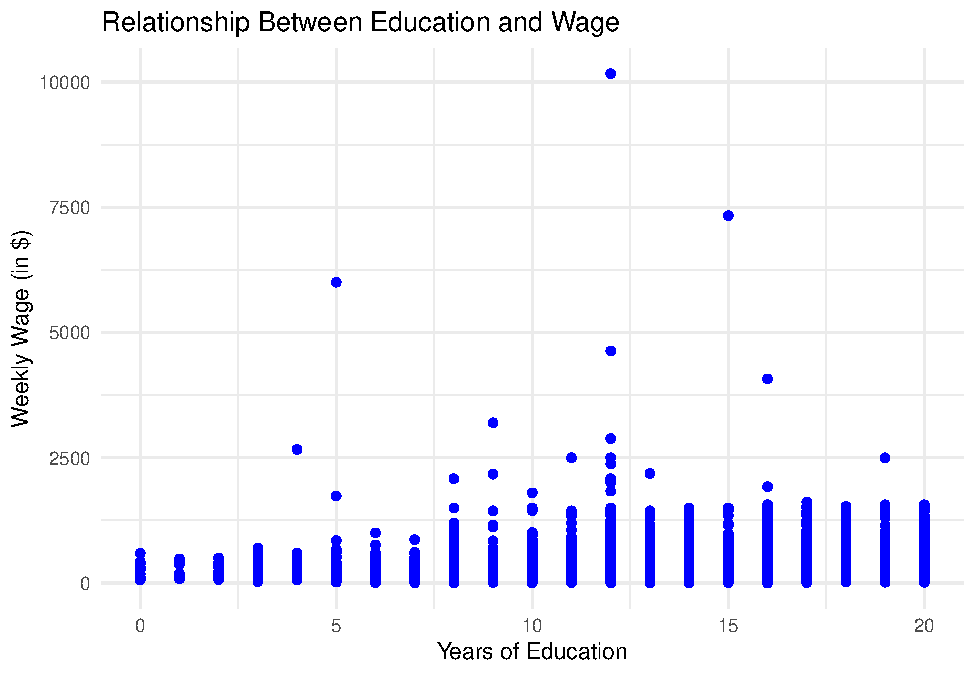
\includegraphics{Data-exploration_files/figure-latex/plot-1.pdf}

\begin{Shaded}
\begin{Highlighting}[]
\CommentTok{\#linear model}

\NormalTok{linear\_model1}\OtherTok{=}\FunctionTok{lm}\NormalTok{(WAGE}\SpecialCharTok{\textasciitilde{}}\NormalTok{ EDUC }\SpecialCharTok{+}\NormalTok{ AGE }\SpecialCharTok{+}\NormalTok{ RACE }\SpecialCharTok{+}\NormalTok{ SMSA }\SpecialCharTok{+}\NormalTok{ MARRIED }\SpecialCharTok{+}\NormalTok{ REGION2 }\SpecialCharTok{+}\NormalTok{ REGION3 }\SpecialCharTok{+}\NormalTok{ REGION4 }\SpecialCharTok{+}\NormalTok{ REGION5 }\SpecialCharTok{+}\NormalTok{ REGION6 }\SpecialCharTok{+}\NormalTok{ REGION7 }\SpecialCharTok{+}\NormalTok{ REGION8 }\SpecialCharTok{+}\NormalTok{ REGION9  }\SpecialCharTok{+}\NormalTok{ QOB2 }\SpecialCharTok{+}\NormalTok{ QOB3 }\SpecialCharTok{+}\NormalTok{ QOB4, }\AttributeTok{data =}\NormalTok{ df)}
\FunctionTok{stargazer}\NormalTok{(linear\_model1,}\AttributeTok{type=}\StringTok{"text"}\NormalTok{,}\AttributeTok{style=}\StringTok{"all"}\NormalTok{)}
\end{Highlighting}
\end{Shaded}

\begin{verbatim}
## 
## =========================================================
##                              Dependent variable:         
##                     -------------------------------------
##                                     WAGE                 
## ---------------------------------------------------------
## EDUC                              26.729***              
##                                    (0.869)               
##                                  t = 30.741              
##                                   p = 0.000              
## AGE                                2.226**               
##                                    (0.953)               
##                                   t = 2.335              
##                                   p = 0.020              
## RACE                             -77.478***              
##                                   (10.229)               
##                                  t = -7.574              
##                                   p = 0.000              
## SMSA                             -63.654***              
##                                    (7.395)               
##                                  t = -8.608              
##                                   p = 0.000              
## MARRIED                           77.927***              
##                                    (8.028)               
##                                   t = 9.706              
##                                   p = 0.000              
## REGION2                           41.204***              
##                                   (13.645)               
##                                   t = 3.020              
##                                   p = 0.003              
## REGION3                           49.071***              
##                                   (13.307)               
##                                   t = 3.688              
##                                  p = 0.0003              
## REGION4                            18.633                
##                                   (15.605)               
##                                   t = 1.194              
##                                   p = 0.233              
## REGION5                             4.120                
##                                   (13.495)               
##                                   t = 0.305              
##                                   p = 0.761              
## REGION6                             7.512                
##                                   (16.126)               
##                                   t = 0.466              
##                                   p = 0.642              
## REGION7                            16.675                
##                                   (14.652)               
##                                   t = 1.138              
##                                   p = 0.256              
## REGION8                            15.916                
##                                   (17.110)               
##                                   t = 0.930              
##                                   p = 0.353              
## REGION9                           63.543***              
##                                   (14.048)               
##                                   t = 4.523              
##                                  p = 0.00001             
## QOB2                               -3.940                
##                                    (7.942)               
##                                  t = -0.496              
##                                   p = 0.620              
## QOB3                                4.786                
##                                    (7.692)               
##                                   t = 0.622              
##                                   p = 0.534              
## QOB4                               -3.725                
##                                    (7.871)               
##                                  t = -0.473              
##                                   p = 0.637              
## Constant                          -80.593*               
##                                   (47.936)               
##                                  t = -1.681              
##                                   p = 0.093              
## ---------------------------------------------------------
## Observations                       10,000                
## R2                                  0.134                
## Adjusted R2                         0.133                
## Residual Std. Error          275.047 (df = 9983)         
## F Statistic         96.743*** (df = 16; 9983) (p = 0.000)
## =========================================================
## Note:                         *p<0.1; **p<0.05; ***p<0.01
\end{verbatim}

\subsubsection{Betekenis coef}\label{betekenis-coef}

EDUC (26.729, p \textless{} 0.001)

A one-year increase in education leads to a \$26.73 increase in wages.
This is highly significant (p = 0.000).

AGE (2.226, p = 0.020) A one-year increase in age increases wages by
\$2.23. Significant at the 5\% level (p = 0.020).

RACE (-77.478, p \textless{} 0.001) Suggests a wage penalty of \$77.48
for certain racial groups (assuming a binary variable where non-white =
1). Highly significant (p = 0.000).

SMSA (-63.654, p \textless{} 0.001) Living in an SMSA (Standard
Metropolitan Statistical Area) is associated with a \$63.65 lower wage.
Significant at p = 0.000.

MARRIED (77.927, p \textless{} 0.001) Being married increases wages by
\$77.93. Highly significant (p = 0.000).

Regional Effects on Wages

Significant Regions: REGION2 (B = 41.204, p = 0.003) REGION3 (B =
49.071, p = 0.0003) REGION9 (B = 63.543, p = 0.00001) These regions have
higher wages compared to the reference region.

Non-Significant Regions: REGION4, REGION5, REGION6, REGION7, REGION8 (p
\textgreater{} 0.05) These regions do not significantly differ from the
reference region in terms of wages.

QOB: being born in Q2 is associated with a \$3.94 lower wage compared to
Q1, Being born in Q3 is associated with a \$4.79 higher wage compared to
Q1, while Being born in Q4 is associated with a \$3.73 lower wage
compared to Q1.None of the QOB coefficients are significant, meaning
quarter of birth does not have a meaningful impact on wages in this
model. The p-values (all \textgreater{} 0.5) suggest that there is no
strong evidence that being born in a particular quarter affects wages

While the model is statistically significant, it explains only 13.4\% of
the variation in wages. Other unobserved factors (e.g.~experience,
skills) likely play a major role.

\begin{Shaded}
\begin{Highlighting}[]
\CommentTok{\# Joint significance test: Test whether AGE, RACE, MARRIED, and SMSA jointly contribute to explaining WAGE.}
\FunctionTok{linearHypothesis}\NormalTok{(linear\_model1, }\FunctionTok{c}\NormalTok{(}\StringTok{"AGE = 0"}\NormalTok{, }\StringTok{"RACE = 0"}\NormalTok{, }\StringTok{"MARRIED = 0"}\NormalTok{, }\StringTok{"SMSA = 0"}\NormalTok{))}
\end{Highlighting}
\end{Shaded}

\begin{verbatim}
## 
## Linear hypothesis test:
## AGE = 0
## RACE = 0
## MARRIED = 0
## SMSA = 0
## 
## Model 1: restricted model
## Model 2: WAGE ~ EDUC + AGE + RACE + SMSA + MARRIED + REGION2 + REGION3 + 
##     REGION4 + REGION5 + REGION6 + REGION7 + REGION8 + REGION9 + 
##     QOB2 + QOB3 + QOB4
## 
##   Res.Df       RSS Df Sum of Sq     F    Pr(>F)    
## 1   9987 773377834                                 
## 2   9983 755224625  4  18153209 59.99 < 2.2e-16 ***
## ---
## Signif. codes:  0 '***' 0.001 '**' 0.01 '*' 0.05 '.' 0.1 ' ' 1
\end{verbatim}

\begin{Shaded}
\begin{Highlighting}[]
\CommentTok{\#Assess whether regional differences are statistically significant.}
\FunctionTok{linearHypothesis}\NormalTok{(linear\_model1, }\FunctionTok{c}\NormalTok{(}\StringTok{"REGION2 = 0"}\NormalTok{,}\StringTok{"REGION3 = 0"}\NormalTok{, }\StringTok{"REGION4 = 0"}\NormalTok{, }\StringTok{"REGION5 = 0"}\NormalTok{, }\StringTok{"REGION6 = 0"}\NormalTok{, }\StringTok{"REGION7 = 0"}\NormalTok{, }\StringTok{"REGION8 = 0"}\NormalTok{, }\StringTok{"REGION9 = 0"}\NormalTok{ ))}
\end{Highlighting}
\end{Shaded}

\begin{verbatim}
## 
## Linear hypothesis test:
## REGION2 = 0
## REGION3 = 0
## REGION4 = 0
## REGION5 = 0
## REGION6 = 0
## REGION7 = 0
## REGION8 = 0
## REGION9 = 0
## 
## Model 1: restricted model
## Model 2: WAGE ~ EDUC + AGE + RACE + SMSA + MARRIED + REGION2 + REGION3 + 
##     REGION4 + REGION5 + REGION6 + REGION7 + REGION8 + REGION9 + 
##     QOB2 + QOB3 + QOB4
## 
##   Res.Df       RSS Df Sum of Sq      F   Pr(>F)    
## 1   9991 759835148                                 
## 2   9983 755224625  8   4610523 7.6181 3.28e-10 ***
## ---
## Signif. codes:  0 '***' 0.001 '**' 0.01 '*' 0.05 '.' 0.1 ' ' 1
\end{verbatim}

Since the p-value is extremely small (\textless0.001), we reject the
null hypothesis. This means that at least one of the region coefficients
is significantly different from zero, implying that region does have a
statistically significant effect on wages.

MKV 1: EDC en AGE zijn stochastic, dummy variables zijn deterministic

\begin{Shaded}
\begin{Highlighting}[]
\FunctionTok{plot}\NormalTok{(linear\_model1}\SpecialCharTok{$}\NormalTok{fitted.values, }\FunctionTok{resid}\NormalTok{(linear\_model1),}
     \AttributeTok{main =} \StringTok{"Residuals vs. Fitted Values"}\NormalTok{,}
     \AttributeTok{xlab =} \StringTok{"Fitted Values"}\NormalTok{,}
     \AttributeTok{ylab =} \StringTok{"Residuals"}\NormalTok{,}
     \AttributeTok{pch =} \DecValTok{16}\NormalTok{, }\AttributeTok{col =} \StringTok{"black"}\NormalTok{)}
\FunctionTok{abline}\NormalTok{(}\AttributeTok{h =} \DecValTok{0}\NormalTok{, }\AttributeTok{lty =} \DecValTok{2}\NormalTok{, }\AttributeTok{col =} \StringTok{"red"}\NormalTok{)  }\CommentTok{\# Add a reference line at zero}
\end{Highlighting}
\end{Shaded}

\includegraphics{Data-exploration_files/figure-latex/unnamed-chunk-2-1.pdf}

\begin{Shaded}
\begin{Highlighting}[]
\CommentTok{\# Updated upstream}


\CommentTok{\# Residuen opslaan}
\NormalTok{residuals }\OtherTok{\textless{}{-}} \FunctionTok{residuals}\NormalTok{(linear\_model1) }
\CommentTok{\# Histogram van de residuen}
\FunctionTok{ggplot}\NormalTok{(}\FunctionTok{data.frame}\NormalTok{(residuals), }\FunctionTok{aes}\NormalTok{(}\AttributeTok{x =}\NormalTok{ residuals)) }\SpecialCharTok{+}
  \FunctionTok{geom\_histogram}\NormalTok{(}\AttributeTok{binwidth =} \DecValTok{5}\NormalTok{, }\AttributeTok{color =} \StringTok{"black"}\NormalTok{, }\AttributeTok{fill =} \StringTok{"blue"}\NormalTok{, }\AttributeTok{alpha =} \FloatTok{0.7}\NormalTok{) }\SpecialCharTok{+}
  \FunctionTok{labs}\NormalTok{(}\AttributeTok{title =} \StringTok{"Histogram van de Residuen"}\NormalTok{, }\AttributeTok{x =} \StringTok{"Residuals"}\NormalTok{, }\AttributeTok{y =} \StringTok{"Frequentie"}\NormalTok{) }\SpecialCharTok{+}
  \FunctionTok{theme\_minimal}\NormalTok{()}
\end{Highlighting}
\end{Shaded}

\includegraphics{Data-exploration_files/figure-latex/unnamed-chunk-3-1.pdf}

\begin{Shaded}
\begin{Highlighting}[]
\CommentTok{\# Q{-}Q plot}
\FunctionTok{qqnorm}\NormalTok{(residuals)}
\FunctionTok{qqline}\NormalTok{(residuals, }\AttributeTok{col =} \StringTok{"red"}\NormalTok{, }\AttributeTok{lwd =} \DecValTok{2}\NormalTok{)}
\end{Highlighting}
\end{Shaded}

\includegraphics{Data-exploration_files/figure-latex/unnamed-chunk-4-1.pdf}

\begin{verbatim}
Jarque Bera Test
\end{verbatim}

data: residuals X-squared = 21719878, df = 2, p-value \textless{}
2.2e-16

Since the p value is small, we reject the null hypothesis .Therefore the
residuals are NOT normally distributed. Implications for OLS: 1)
Unbiasedness: Non-normal residuals do not affect the unbiasedness of OLS
estimators as long as key assumptions (like linearity, exogeneity of
regressors, and zero-mean error term) are satisfied

\begin{verbatim}
  2) Efficiency:
  OLS estimators may lose their efficiency because normality of residuals is necessary for OLS to be the Best Linear Unbiased Estimator  (BLUE) under the Gauss-Markov assumptions.
  
  3) Hypothesis Testing:
  The validity of tests (e.g., (t)-tests and (F)-tests) and confidence intervals relies on the normality assumption. Non-normal residuals         can lead to incorrect p-values
  
  4) Heteroscedasticity or Outliers:
  Non-normality can signal issues like heteroscedasticity (non-constant error variance), the presence of outliers, or omitted variable bias. 
  
  Remediation:
  Based on the histogram and Q-Q Plot which is slightly right skewed, we can conclude that the residuals deviate slightly from normality, so OLS may still perform adequately, particularly in our large sample where asymptotic normality applies.
  
  
  
\end{verbatim}

Gauss-Markov assumptions:

Assumption 1: Linearity in the parameters: CHECK

Assumption 2a: The X -values are fixed over repeated sampling (fixed
regressor model) FAIL

Correlation between explanatory variables and error terms: residuals
EDUC AGE RACE SMSA residuals 1.000000e+00 7.941822e-16 6.055269e-15
2.730699e-16 7.292579e-17 EDUC 7.941822e-16 1.000000e+00 -6.950629e-02
-1.519529e-01 -1.490703e-01 AGE 6.055269e-15 -6.950629e-02 1.000000e+00
-5.148653e-03 -2.085355e-02 RACE 2.730699e-16 -1.519529e-01
-5.148653e-03 1.000000e+00 -3.556389e-02 SMSA 7.292579e-17 -1.490703e-01
-2.085355e-02 -3.556389e-02 1.000000e+00 MARRIED -1.401804e-15
1.919836e-02 2.080998e-02 -1.132829e-01 4.064474e-02 REGION2
8.966308e-17 3.571736e-02 8.497716e-03 1.409293e-02 -1.039187e-01
REGION3 -1.027672e-16 -3.083976e-02 5.358420e-03 -2.390864e-02
-2.447606e-02 REGION4 2.251761e-17 -5.788070e-04 -1.490758e-02
-4.990867e-02 1.178779e-01 REGION5 6.142732e-17 -4.295309e-02
-1.217907e-02 9.147281e-02 1.940650e-02 REGION6 1.531221e-16
-8.442759e-02 8.312525e-03 3.957577e-02 1.134396e-01 REGION7
7.960569e-17 -3.280617e-02 3.156501e-03 8.728591e-03 -1.074680e-02
REGION8 -1.504773e-17 2.845508e-02 -2.617902e-02 -4.361064e-02
7.119329e-02 REGION9 9.619108e-17 1.046830e-01 1.483814e-03
-3.011996e-02 -7.742498e-02 QOB2 -1.301029e-16 9.299750e-03
-5.128026e-02 2.146201e-02 -5.371836e-03 QOB3 -2.411359e-16
-1.429164e-02 -5.001583e-02 -6.116495e-03 -1.219575e-02 QOB4
-1.066005e-16 3.457342e-02 -5.119262e-02 -1.342702e-02 4.891620e-04
MARRIED REGION2 REGION3 REGION4 REGION5 residuals -1.401804e-15
8.966308e-17 -1.027672e-16 2.251761e-17 6.142732e-17 EDUC 1.919836e-02
3.571736e-02 -3.083976e-02 -5.788070e-04 -4.295309e-02 AGE 2.080998e-02
8.497716e-03 5.358420e-03 -1.490758e-02 -1.217907e-02 RACE -1.132829e-01
1.409293e-02 -2.390864e-02 -4.990867e-02 9.147281e-02 SMSA 4.064474e-02
-1.039187e-01 -2.447606e-02 1.178779e-01 1.940650e-02 MARRIED
1.000000e+00 -3.692641e-03 1.393788e-02 2.088136e-02 4.255528e-03
REGION2 -3.692641e-03 1.000000e+00 -2.134547e-01 -1.219235e-01
-2.013995e-01 REGION3 1.393788e-02 -2.134547e-01 1.000000e+00
-1.382750e-01 -2.284097e-01 REGION4 2.088136e-02 -1.219235e-01
-1.382750e-01 1.000000e+00 -1.304656e-01 REGION5 4.255528e-03
-2.013995e-01 -2.284097e-01 -1.304656e-01 1.000000e+00 REGION6
1.773853e-02 -1.134428e-01 -1.286569e-01 -7.348769e-02 -1.213908e-01
REGION7 7.148294e-03 -1.442097e-01 -1.635501e-01 -9.341835e-02
-1.543133e-01 REGION8 2.095671e-02 -9.889841e-02 -1.121620e-01
-6.406592e-02 -1.058274e-01 REGION9 -6.080853e-02 -1.665132e-01
-1.888447e-01 -1.078665e-01 -1.781794e-01 QOB2 1.051784e-02 1.428433e-02
1.907353e-03 6.956636e-03 -1.256816e-02 QOB3 9.110159e-03 -4.679173e-03
-1.264083e-02 1.963180e-03 -4.200310e-03 QOB4 -1.597186e-02 8.713668e-03
2.727022e-03 -2.282908e-02 1.192933e-02 REGION6 REGION7 REGION8 REGION9
QOB2 residuals 1.531221e-16 7.960569e-17 -1.504773e-17 9.619108e-17
-1.301029e-16 EDUC -8.442759e-02 -3.280617e-02 2.845508e-02 1.046830e-01
9.299750e-03 AGE 8.312525e-03 3.156501e-03 -2.617902e-02 1.483814e-03
-5.128026e-02 RACE 3.957577e-02 8.728591e-03 -4.361064e-02 -3.011996e-02
2.146201e-02 SMSA 1.134396e-01 -1.074680e-02 7.119329e-02 -7.742498e-02
-5.371836e-03 MARRIED 1.773853e-02 7.148294e-03 2.095671e-02
-6.080853e-02 1.051784e-02 REGION2 -1.134428e-01 -1.442097e-01
-9.889841e-02 -1.665132e-01 1.428433e-02 REGION3 -1.286569e-01
-1.635501e-01 -1.121620e-01 -1.888447e-01 1.907353e-03 REGION4
-7.348769e-02 -9.341835e-02 -6.406592e-02 -1.078665e-01 6.956636e-03
REGION5 -1.213908e-01 -1.543133e-01 -1.058274e-01 -1.781794e-01
-1.256816e-02 REGION6 1.000000e+00 -8.692041e-02 -5.960966e-02
-1.003635e-01 -3.520934e-03 REGION7 -8.692041e-02 1.000000e+00
-7.577645e-02 -1.275832e-01 -2.379928e-02 REGION8 -5.960966e-02
-7.577645e-02 1.000000e+00 -8.749605e-02 -3.128284e-04 REGION9
-1.003635e-01 -1.275832e-01 -8.749605e-02 1.000000e+00 8.276435e-03 QOB2
-3.520934e-03 -2.379928e-02 -3.128284e-04 8.276435e-03 1.000000e+00 QOB3
-4.741142e-03 3.014449e-02 -1.156843e-02 8.549162e-03 -3.352226e-01 QOB4
-3.897055e-03 -1.307343e-03 4.850047e-03 -8.469705e-03 -3.151392e-01
QOB3 QOB4 residuals -2.411359e-16 -1.066005e-16 EDUC -1.429164e-02
3.457342e-02 AGE -5.001583e-02 -5.119262e-02 RACE -6.116495e-03
-1.342702e-02 SMSA -1.219575e-02 4.891620e-04 MARRIED 9.110159e-03
-1.597186e-02 REGION2 -4.679173e-03 8.713668e-03 REGION3 -1.264083e-02
2.727022e-03 REGION4 1.963180e-03 -2.282908e-02 REGION5 -4.200310e-03
1.192933e-02 REGION6 -4.741142e-03 -3.897055e-03 REGION7 3.014449e-02
-1.307343e-03 REGION8 -1.156843e-02 4.850047e-03 REGION9 8.549162e-03
-8.469705e-03 QOB2 -3.352226e-01 -3.151392e-01 QOB3 1.000000e+00
-3.431338e-01 QOB4 -3.431338e-01 1.000000e+00

\begin{Shaded}
\begin{Highlighting}[]
\FunctionTok{print}\NormalTok{(}\FunctionTok{mean}\NormalTok{(residuals))}
\end{Highlighting}
\end{Shaded}

\begin{verbatim}
## [1] -4.164089e-15
\end{verbatim}

\begin{Shaded}
\begin{Highlighting}[]
\FunctionTok{print}\NormalTok{(}\FunctionTok{t.test}\NormalTok{(residuals, }\AttributeTok{mu =} \DecValTok{0}\NormalTok{))}
\end{Highlighting}
\end{Shaded}

\begin{verbatim}
## 
##  One Sample t-test
## 
## data:  residuals
## t = -1.5152e-15, df = 9999, p-value = 1
## alternative hypothesis: true mean is not equal to 0
## 95 percent confidence interval:
##  -5.387167  5.387167
## sample estimates:
##     mean of x 
## -4.164089e-15
\end{verbatim}

\begin{Shaded}
\begin{Highlighting}[]
\ControlFlowTok{if}\NormalTok{ (show\_interpretation) \{}
  \FunctionTok{cat}\NormalTok{(}\StringTok{"Assumption 3: The expected V value of the error terms is zero: CHECK"}\NormalTok{)}
\NormalTok{\}}
\end{Highlighting}
\end{Shaded}

\begin{verbatim}
## Assumption 3: The expected V value of the error terms is zero: CHECK
\end{verbatim}

\begin{Shaded}
\begin{Highlighting}[]
\FunctionTok{bptest}\NormalTok{(linear\_model1)}
\end{Highlighting}
\end{Shaded}

\begin{verbatim}
## 
##  studentized Breusch-Pagan test
## 
## data:  linear_model1
## BP = 8.9621, df = 16, p-value = 0.915
\end{verbatim}

euuhhh , deze test zegt dat er geen heteroskedasticity is , maar onze
residuals zijn wel niet nrml verdeeld lol . geen idee hoe ik verder moet

\end{document}
